\section{Weiterentwicklung}

In der zweiten Phase des Projekts soll die Funktionalität des KSM erweitert werden. Besonderes Augenmerk liegt hierbei auf der Verbesserung der Anzeige, welche Knoten im aktiven/passiven, oder kritischen Bereich liegen. Diese Anzeige wird intern auch Sum-Chart genannt. Hier wurde bereits in einer der letzten Studienarbeiten von Frau Klein angefangen, es dem Benutzer zu ermöglichen, Bereiche zu definieren und zu markieren \cite{bib:klein}. Bereiche waren in diesem Fall Ellipsen, die vom Benutzer aufgezogen wurden. Je größer diese wurden, desto transparenter wurde die Füllfarbe.
\begin{figure}[h]
	\centering
	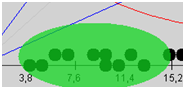
\includegraphics[width=0.4\textwidth]{pictures/ellipse.png}
	\caption{Bereichsmarkierung nach Klein \cite{bib:klein}}
	\label{magic-cycle}
\end{figure}

Nach Evaluation dieser Implementierung kam Herr Professor Schubert zu dem Schluss, dass Ellipsen auf der einen Seite zu unflexibel sind, um einen Bereich adäquat ausbilden zu können. Auf der anderen Seite jedoch auf keinerlei Begrenzungen, wie zum Beispiel aktiv, passiv Rücksicht nehmen. Dazu wurde die Füllfarbe trotz Transparenz teilweise als zu deckend empfunden.

\subsection{Anforderungen}

Die neuen Anforderungen an eine Bereichsmarkierung lauteten nach diesen Erkenntnissen wie folgt:
\begin{itemize}
  \item Der Benutzer muss in der Lage sein, einen Bereich mittels Eckpunkten definieren zu können
  \item Es dürfen beliebig viele Eckpunkte sein
  \item Die Eckpunkte dürfen nur auf Bereits vorhandenen Linien laufen:
  \begin{itemize}
    \item X-Achse
    \item Y-Achse
    \item Diagrammbegrenzungen parallel zu X- oder Y-Achse
    \item Q-Achsen zur Abgrenzung der aktiven/passiven Bereiche, sowie Q = 1 als Mitte
    \item Hyperbeln zur Markierung des stabilen/kritischen Bereichs
  \end{itemize}
  \item Punkte (Knoten des System Graphen), die innerhalb des markierten Bereichs liegen, müssen aufgelistet werden
  \item Die Füllfarbe des Bereichs soll transparenter sein, als bisher
\end{itemize}

Dazu wurde noch von den Projektmitgliedern entschieden, dass erstellte Bereiche benannt werden sollen. Dieser Name soll innerhalb des Bereichs sichtbar sein.
